% pyMOFL: A Composable Optimization Benchmark Library for Python
% arXiv preprint
\documentclass[11pt,a4paper]{article}

% ---- Packages ----
\usepackage[utf8]{inputenc}
\usepackage[T1]{fontenc}
\usepackage{amsmath,amssymb}
\usepackage{booktabs}
\usepackage{graphicx}
\usepackage{hyperref}
\usepackage{xcolor}
\usepackage{listings}
\usepackage{algorithm}
\usepackage{algpseudocode}
\usepackage[margin=1in]{geometry}
\usepackage{natbib}
\usepackage{enumitem}
\usepackage{caption}
\usepackage{subcaption}
\usepackage{tikz}
\usetikzlibrary{arrows.meta,positioning,shapes.geometric,fit}

% ---- Listing style ----
\lstset{
  language=Python,
  basicstyle=\ttfamily\small,
  keywordstyle=\color{blue!80!black},
  commentstyle=\color{green!50!black},
  stringstyle=\color{red!60!black},
  showstringspaces=false,
  breaklines=true,
  frame=single,
  framesep=3pt,
  xleftmargin=1em,
  numbers=left,
  numberstyle=\tiny\color{gray},
  numbersep=5pt,
  tabsize=4,
  captionpos=b,
}

% ---- Macros ----
\newcommand{\pymofl}{\textsc{pyMOFL}}
\newcommand{\numpy}{\textsc{NumPy}}
\newcommand{\R}{\mathbb{R}}

\title{\pymofl{}: A Composable Optimization Benchmark Library for Python}

\author{
  Travis Silvers\\
  \texttt{firestrand@users.noreply.github.com}\\
  \url{https://github.com/firestrand/pyMOFL}
}

\date{}

\begin{document}

\maketitle

% ============================================================
\begin{abstract}
We present \pymofl{}, an open-source Python library for constructing and
evaluating optimization benchmark functions through functional composition.
Unlike existing benchmark libraries that rely on class inheritance hierarchies
to combine transformations with base functions, \pymofl{} decouples
transformations from objective functions entirely: shifts, rotations, scaling,
bias, and noise are pure callable objects composed around base functions via a
generic pipeline. A declarative JSON configuration layer drives construction of
arbitrarily complex benchmarks---including all 25 functions of the CEC\,2005
special session---without writing function-specific code. The library provides
47 benchmark function implementations, 14 transformation types, weighted
composition and hybrid function abstractions, and a modular factory system that
maps configuration trees to executable function objects. All operations are
vectorized through \numpy{}, supporting efficient batch evaluation. \pymofl{}
is available under the MIT license at
\url{https://github.com/firestrand/pyMOFL} and via PyPI.
\end{abstract}

\noindent\textbf{Keywords:} optimization benchmarks, metaheuristics, benchmark functions,
CEC\,2005, function composition, Python

% ============================================================
\section{Introduction}\label{sec:intro}

Benchmark functions are essential infrastructure for optimization research.
They provide controlled, reproducible landscapes on which algorithms can be
compared with respect to convergence speed, solution quality, scalability, and
robustness to problem characteristics such as multimodality, non-separability,
ill-conditioning, and noise~\citep{Jamil2013}. Standardized benchmark suites,
most notably the series organized by the Congress on Evolutionary Computation
(CEC)~\citep{Suganthan2005}, have become the \emph{de facto} protocol for
evaluating metaheuristic optimizers.

Despite decades of use, the software implementations of these benchmarks remain
fragmented. Researchers frequently re-implement functions from scratch,
introducing subtle discrepancies in transformation order, rotation convention,
or bias handling that compromise reproducibility. Existing libraries such as
Opfunu~\citep{VanThieu2024}, COCO/BBOB~\citep{Hansen2021}, and
Benchmarks.jl~\citep{benchmarksjl} vary in the degree to which they expose the
internal composition of transformed functions, making it difficult to extend
suites or verify intermediate transformation steps.

\pymofl{} addresses these challenges through three design principles:

\begin{enumerate}[leftmargin=*,nosep]
  \item \textbf{Composition over inheritance.} Transformations are
    pure callable objects---not subclasses of the objective function base
    class---composed via a generic pipeline (\texttt{ComposedFunction}).
  \item \textbf{Declarative configuration.} A JSON configuration tree is the
    single source of truth for any benchmark variant. The nesting structure
    directly encodes the transformation application order.
  \item \textbf{Vectorized evaluation.} All transforms and functions support
    batch evaluation through \numpy{} array operations, enabling efficient
    use in population-based algorithms.
\end{enumerate}

The remainder of this paper is organized as follows.
Section~\ref{sec:related} surveys related work.
Section~\ref{sec:architecture} describes the library architecture.
Section~\ref{sec:functions} catalogs the implemented benchmark functions.
Section~\ref{sec:transforms} details the transformation pipeline.
Section~\ref{sec:compositions} explains weighted composition and hybrid function
abstractions.
Section~\ref{sec:factory} presents the config-driven factory system.
Section~\ref{sec:cec2005} demonstrates CEC\,2005 suite coverage.
Section~\ref{sec:usage} provides usage examples.
Section~\ref{sec:quality} discusses testing and quality assurance.
Section~\ref{sec:conclusion} concludes.

% ============================================================
\section{Related Work}\label{sec:related}

Several software packages provide optimization benchmark functions for
research. We briefly compare the most prominent.

\textbf{Opfunu}~\citep{VanThieu2024} offers over 500 functions spanning
CEC\,2005--2022 and traditional benchmarks. It uses a class-inheritance model
in which each CEC function is a standalone class with hard-coded
transformations. This simplifies lookup but couples transformation logic to
specific functions, making it difficult to recombine transforms independently.

\textbf{COCO/BBOB}~\citep{Hansen2021} provides a carefully designed testbed
for black-box optimization with automated performance assessment. COCO is
implemented in C with Python bindings, emphasizing runtime performance but
offering limited user-level extensibility for custom function composition.

\textbf{SciPy \texttt{optimize}}~\citep{Virtanen2020} includes a small
collection of test functions but is not designed as a comprehensive benchmark
library.

\textbf{Benchmarks.jl}~\citep{benchmarksjl} targets the Julia ecosystem with
a collection of classical test functions. Like Opfunu, transformations are
embedded within individual function implementations.

Table~\ref{tab:comparison} summarizes key differences. \pymofl{}'s
distinguishing contribution is the separation of concerns between base
functions, transformations, and composition logic, enabled by a config-driven
factory pipeline.

\begin{table}[t]
\centering
\caption{Comparison of optimization benchmark libraries.}
\label{tab:comparison}
\begin{tabular}{@{}lccccc@{}}
\toprule
& \textbf{Language} & \textbf{Functions} & \textbf{CEC Suites} & \textbf{Composable} & \textbf{Config-driven} \\
\midrule
Opfunu        & Python & 500+    & 2005--2022 & No  & No  \\
COCO/BBOB     & C/Py   & 24/suite & BBOB       & No  & No  \\
SciPy         & Python & $\sim$15 & ---        & No  & No  \\
Benchmarks.jl & Julia  & $\sim$30 & ---        & No  & No  \\
\textbf{\pymofl{}} & \textbf{Python} & \textbf{47} & \textbf{2005} & \textbf{Yes} & \textbf{Yes} \\
\bottomrule
\end{tabular}
\end{table}

% ============================================================
\section{Architecture}\label{sec:architecture}

\pymofl{} is organized around four layers, shown in
Figure~\ref{fig:architecture}: base functions, transformations, compositions,
and a factory system that assembles them from configuration.

\begin{figure}[t]
\centering
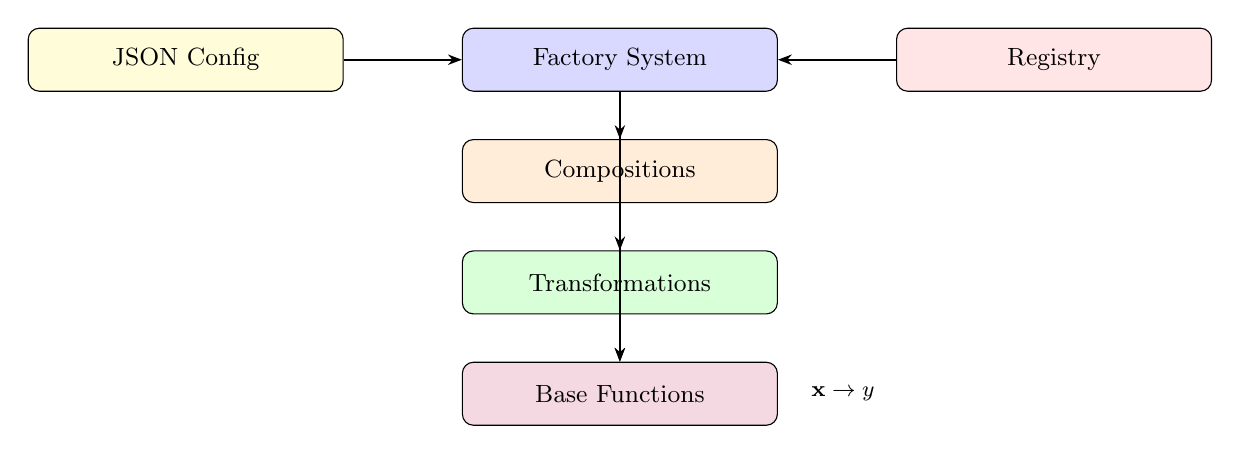
\begin{tikzpicture}[
    box/.style={draw, rounded corners, minimum width=4cm, minimum height=0.8cm, align=center, font=\small},
    layer/.style={draw, dashed, rounded corners, inner sep=8pt, fill=#1!5},
    arr/.style={-{Stealth[length=5pt]}, thick},
    node distance=0.6cm
  ]
  % Layers
  \node[box, fill=blue!15] (factory) {Factory System};
  \node[box, fill=orange!15, below=of factory] (comps) {Compositions};
  \node[box, fill=green!15, below=of comps] (transforms) {Transformations};
  \node[box, fill=purple!15, below=of transforms] (base) {Base Functions};

  % JSON
  \node[box, fill=yellow!15, left=1.5cm of factory] (json) {JSON Config};

  % Registry
  \node[box, fill=red!10, right=1.5cm of factory] (registry) {Registry};

  % Arrows
  \draw[arr] (json) -- (factory);
  \draw[arr] (registry) -- (factory);
  \draw[arr] (factory) -- (comps);
  \draw[arr] (factory) -- (transforms);
  \draw[arr] (comps) -- (base);
  \draw[arr] (transforms) -- (base);

  % Evaluation flow label
  \node[font=\footnotesize\itshape, right=0.3cm of base] {$\mathbf{x} \to y$};
\end{tikzpicture}
\caption{High-level architecture. The factory system reads JSON configuration
and the function registry to assemble compositions of transformations and base
functions. Evaluation flows bottom-up: input transforms are applied to
$\mathbf{x}$, the base function is evaluated, and output transforms produce
the final scalar $y$.}
\label{fig:architecture}
\end{figure}

\subsection{Design Principles}

\paragraph{Composition over inheritance.}
Optimization benchmark suites typically require the same base function
(e.g., Sphere) to appear in multiple variants: shifted, rotated, shifted
\emph{and} rotated, with noise, with bias, etc. An inheritance-based design
leads to a combinatorial explosion of subclasses. \pymofl{} instead treats
transformations as independent, composable units:

\begin{equation}
f_{\text{composed}}(\mathbf{x}) = T_{\text{out}} \circ f_{\text{base}} \circ T_{\text{in}}(\mathbf{x})
\label{eq:composition}
\end{equation}

\noindent where $T_{\text{in}}$ and $T_{\text{out}}$ are ordered sequences of
vector and scalar transforms, respectively.

\paragraph{Bounds as metadata.}
Unlike libraries that enforce box constraints within the function evaluation,
\pymofl{} treats bounds as pure metadata
(\texttt{Bounds} frozen dataclass with \texttt{low}, \texttt{high}, \texttt{mode},
\texttt{qtype}, \texttt{step}). Enforcement or quantization is opt-in via
the \texttt{Quantized} wrapper. This prevents the benchmark implementation from
interfering with the optimizer's constraint-handling strategy.

\paragraph{Single source of truth.}
Each benchmark suite is defined by a JSON configuration file. The CEC\,2005
suite, for example, is encoded in a single \texttt{cec2005\_suite.json} file
that specifies all 25 functions across all supported dimensions (2, 10, 30, 50).
Adding a new suite (e.g., BBOB) requires only a new JSON file and any associated
data files---no code changes.

% ============================================================
\section{Benchmark Functions}\label{sec:functions}

\pymofl{} provides 47 benchmark function classes spanning classical unimodal,
multimodal, and engineering design problems. Each class inherits from
\texttt{OptimizationFunction} and implements the abstract \texttt{evaluate(x)}
method. Table~\ref{tab:functions} summarizes the catalog.

\begin{table}[t]
\centering
\caption{Benchmark functions implemented in \pymofl{}, grouped by category.}
\label{tab:functions}
\small
\begin{tabular}{@{}llp{8.5cm}@{}}
\toprule
\textbf{Category} & \textbf{Count} & \textbf{Functions} \\
\midrule
Unimodal & 11 &
  Sphere, Rosenbrock, Schwefel\,1.2, Schwefel\,2.6, Schwefel\,2.13,
  High-Conditioned Elliptic, Dixon--Price, Powell (3 variants),
  Sum of Different Powers \\
\addlinespace
Multimodal & 27 &
  Ackley (4 variants), Rastrigin, Griewank, Weierstrass, Katsuura, Levy,
  Zakharov, Alpine (2), Schaffer (6 variants), Schwefel\,2.4/2.20--2.26/2.36,
  Lunacek Bi-Rastrigin, Easom, Goldstein--Price, McCormick, Matyas,
  HappyCat, HGBat \\
\addlinespace
Composed & 2 &
  Griewank-of-Rosenbrock (F8F2), Expanded Schaffer\,F6 \\
\addlinespace
Engineering & 4 &
  Compression Spring, Gear Train, Network, Lennard-Jones \\
\addlinespace
Utility & 3 &
  Step, Tripod, Max Absolute, Different Powers, Perm, Himmelblau, Branin (2),
  Bent Cigar, Discus \\
\bottomrule
\end{tabular}
\end{table}

All functions are registered with the global \texttt{FunctionRegistry} at
import time via a \texttt{@register} decorator and automatic submodule scanning
(\texttt{scan\_package}). Each function is accessible by one or more string
aliases (e.g., \texttt{"sphere"}, \texttt{"Sphere"}), enabling symbolic lookup
from configuration files.

The base class provides:
\begin{itemize}[nosep]
  \item \texttt{evaluate(x: ndarray) -> float}: single-point evaluation with input validation.
  \item \texttt{evaluate\_batch(X: ndarray) -> ndarray}: batch evaluation (default loops; overridden with vectorized implementations in concrete classes).
  \item \texttt{\_\_call\_\_}: delegates to \texttt{evaluate} with validation.
  \item Metadata properties: \texttt{dimension}, \texttt{initialization\_bounds}, \texttt{operational\_bounds}.
\end{itemize}

% ============================================================
\section{Transformation Pipeline}\label{sec:transforms}

Transformations are the core mechanism for constructing benchmark variants.
\pymofl{} defines two abstract base classes for transforms:

\begin{itemize}[nosep]
  \item \texttt{VectorTransform}: $\R^d \to \R^d$ (input transforms)
  \item \texttt{ScalarTransform}: $\R \to \R$ (output transforms)
\end{itemize}

Both are pure callables---they carry parameters but are not
\texttt{OptimizationFunction} subclasses. Table~\ref{tab:transforms} lists all
implemented transforms.

\begin{table}[t]
\centering
\caption{Transformation types in \pymofl{}.}
\label{tab:transforms}
\small
\begin{tabular}{@{}llll@{}}
\toprule
\textbf{Type} & \textbf{Class} & \textbf{Category} & \textbf{Mathematical Operation} \\
\midrule
Shift     & \texttt{ShiftTransform}     & Vector & $\mathbf{x}' = \mathbf{x} - \mathbf{o}$ \\
Rotate    & \texttt{RotateTransform}    & Vector & $\mathbf{x}' = \mathbf{M}^\top \mathbf{x}$ \\
Scale     & \texttt{ScaleTransform}     & Vector & $\mathbf{x}' = \mathbf{x} / \lambda$ \\
Offset    & \texttt{OffsetTransform}    & Vector & $\mathbf{x}' = \mathbf{x} + \mathbf{v}$ \\
Non-continuous & \texttt{NonContinuousTransform} & Vector & $x_i' = \lfloor 2x_i + 0.5 \rfloor / 2$ \\
Indexed shift  & \texttt{IndexedShiftTransform}  & Vector & Shift on selected dimensions \\
Indexed scale  & \texttt{IndexedScaleTransform}  & Vector & Scale on selected dimensions \\
Indexed rotate & \texttt{IndexedRotateTransform} & Vector & Rotate on selected dimensions \\
\midrule
Bias      & \texttt{BiasTransform}      & Scalar & $y' = y + b$ \\
Noise     & \texttt{NoiseTransform}     & Scalar & $y' = y \cdot (1 + \epsilon)$ \\
Normalize & \texttt{NormalizeTransform}  & Scalar & $y' = y \cdot C / f_{\max}$ \\
Quantize  & \texttt{Quantized}          & Special & Bounds enforcement + discretization \\
\bottomrule
\end{tabular}
\end{table}

\subsection{ComposedFunction}

\texttt{ComposedFunction} is the primary composition mechanism. It is itself an
\texttt{OptimizationFunction}, wrapping a base function with ordered sequences
of input and output transforms:

\begin{lstlisting}[caption={ComposedFunction evaluation flow.},label=lst:composed]
class ComposedFunction(OptimizationFunction):
    def evaluate(self, x):
        z = x
        for t in self.input_transforms:
            z = t(z)                    # VectorTransform chain
        y = self.base_function.evaluate(z)
        for t in self.output_transforms:
            y = t(y)                    # ScalarTransform chain
        return y
\end{lstlisting}

The batch evaluation path applies each transform to the full matrix before
passing to the next stage, preserving \numpy{} vectorization:

\begin{equation}
\mathbf{Y} = T_{\text{out}}^{(m)} \circ \cdots \circ T_{\text{out}}^{(1)} \circ
f_{\text{base}} \circ
T_{\text{in}}^{(k)} \circ \cdots \circ T_{\text{in}}^{(1)}(\mathbf{X})
\label{eq:batch}
\end{equation}

\noindent where $\mathbf{X} \in \R^{n \times d}$ is a batch of $n$ input vectors.

% ============================================================
\section{Composition and Hybrid Functions}\label{sec:compositions}

Beyond simple transform chains, \pymofl{} supports two higher-order
composition patterns required by CEC\,2005 functions F15--F25.

\subsection{Weighted Composition}

\texttt{WeightedComposition} combines $K$ component functions using
distance-based Gaussian weights:

\begin{equation}
f(\mathbf{x}) = \sum_{i=1}^{K} w_i(\mathbf{x}) \cdot \left[
  C_i \cdot \frac{f_i(\mathbf{x})}{f_{\max,i}} + b_i
\right] + b_{\text{global}}
\label{eq:weighted}
\end{equation}

\noindent where the weight for component $i$ is:

\begin{equation}
w_i(\mathbf{x}) = \frac{\hat{w}_i}{\sum_{j=1}^{K} \hat{w}_j}, \quad
\hat{w}_i = \exp\!\left(-\frac{\|\mathbf{x} - \mathbf{o}_i\|^2}{2\sigma_i^2 d}\right)
\label{eq:weights}
\end{equation}

Here $\mathbf{o}_i$ is the optimum of component $i$, $\sigma_i$ controls the
basin width, $C_i$ is a normalization constant, $f_{\max,i}$ is the maximum
function value used for normalization (pre-computed at a canonical point), and
$b_i$ is a per-component bias. Optional dominance suppression amplifies the
weight of the nearest component, creating sharper transitions between basins.

Each component is a fully self-contained \texttt{ComposedFunction} with its own
transform chain. The raw input $\mathbf{x}$ (without composition-level
transforms) is used for distance-based weighting, ensuring weight computation
reflects the true distance in the original search space.

\subsection{Hybrid Function}

\texttt{HybridFunction} partitions the input vector $\mathbf{x} \in \R^d$ into
$K$ disjoint subvectors $\mathbf{x}_{[s_i:e_i]}$, each evaluated by a
different component:

\begin{equation}
f(\mathbf{x}) = \sum_{i=1}^{K} \alpha_i \cdot f_i(\mathbf{x}_{[s_i:e_i]})
\label{eq:hybrid}
\end{equation}

\noindent where $\alpha_i$ are optional weights and $(s_i, e_i)$ define the
partition boundaries.

% ============================================================
\section{Config-Driven Factory System}\label{sec:factory}

A central design goal of \pymofl{} is that benchmark construction should be
data-driven. The factory system translates JSON configuration trees into
executable function objects through five specialized modules.

\subsection{Configuration Structure}

The JSON configuration uses a nested structure in which the outermost wrapper
in the tree corresponds to the last transformation applied during evaluation:

\begin{lstlisting}[language={},caption={JSON configuration for CEC\,2005 F03 (Shifted Rotated High-Conditioned Elliptic).},label=lst:config]
{
  "type": "bias",
  "parameters": {"value": -450.0},
  "function": {
    "type": "rotate",
    "parameters": {"matrix": "f03/matrix_rotation_D{dim}.txt"},
    "function": {
      "type": "shift",
      "parameters": {"vector": "f03/vector_shift_D{dim}.txt"},
      "function": {
        "type": "high_conditioned_elliptic",
        "parameters": {"dimension": 10}
      }
    }
  }
}
\end{lstlisting}

This nesting directly encodes the evaluation order: \texttt{shift} is applied
first to $\mathbf{x}$, then \texttt{rotate}, then the base function is
evaluated, then \texttt{bias} is added to the result. The \texttt{\{dim\}}
placeholder is resolved at construction time based on the requested dimension.

\subsection{Factory Modules}

The factory is decomposed into five focused modules (Figure~\ref{fig:factory}):

\begin{description}[nosep,leftmargin=1em]
  \item[\texttt{DataLoader}] Loads shift vectors and rotation matrices from
    text files, supporting dimension-templated filenames.
  \item[\texttt{ConfigParser}] Recursively parses the nested JSON tree,
    collecting transforms in application order and extracting the base function
    specification.
  \item[\texttt{TransformBuilder}] Instantiates \texttt{VectorTransform} and
    \texttt{ScalarTransform} objects from (type, parameters) tuples, loading
    data files as needed.
  \item[\texttt{CompositionBuilder}] Assembles weighted compositions with
    per-component transform chains, optimum loading, and $f_{\max}$
    pre-computation.
  \item[\texttt{FunctionFactory}] Thin orchestrator that delegates to the above
    modules and returns a \texttt{ComposedFunction} or
    \texttt{WeightedComposition}.
\end{description}

\begin{figure}[t]
\centering
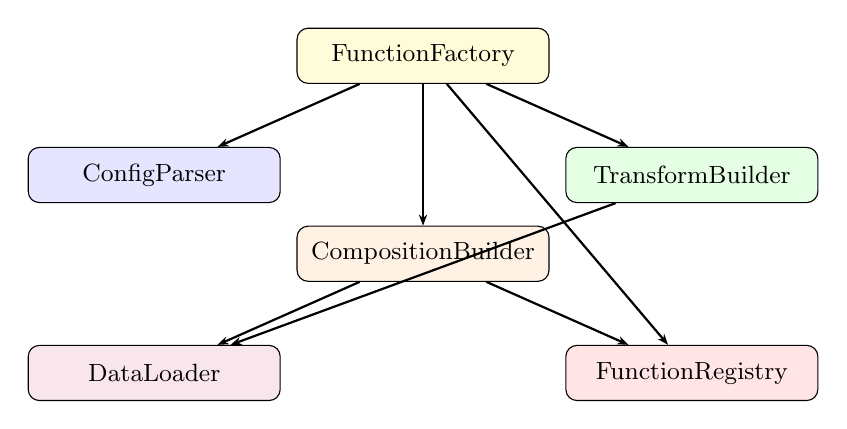
\begin{tikzpicture}[
    box/.style={draw, rounded corners, minimum width=3.2cm, minimum height=0.7cm, align=center, font=\small},
    arr/.style={-{Stealth[length=4pt]}, thick},
    node distance=0.5cm and 1.2cm
  ]
  \node[box, fill=yellow!15] (ff) {FunctionFactory};
  \node[box, fill=blue!10, below left=0.8cm and 0.2cm of ff] (cp) {ConfigParser};
  \node[box, fill=green!10, below right=0.8cm and 0.2cm of ff] (tb) {TransformBuilder};
  \node[box, fill=orange!10, below=1.8cm of ff] (cb) {CompositionBuilder};
  \node[box, fill=purple!10, below left=0.8cm and 0.2cm of cb] (dl) {DataLoader};
  \node[box, fill=red!10, below right=0.8cm and 0.2cm of cb] (reg) {FunctionRegistry};

  \draw[arr] (ff) -- (cp);
  \draw[arr] (ff) -- (tb);
  \draw[arr] (ff) -- (cb);
  \draw[arr] (tb) -- (dl);
  \draw[arr] (cb) -- (dl);
  \draw[arr] (cb) -- (reg);
  \draw[arr] (ff) -- (reg);
\end{tikzpicture}
\caption{Factory module decomposition. \texttt{FunctionFactory} orchestrates
parsing, transform construction, composition building, and registry lookup.}
\label{fig:factory}
\end{figure}

% ============================================================
\section{CEC\,2005 Suite Coverage}\label{sec:cec2005}

\pymofl{} provides complete coverage of the CEC\,2005 special session on
real-parameter optimization~\citep{Suganthan2005}, all 25 functions across
dimensions 2, 10, 30, and 50. The suite is defined entirely in
\texttt{cec2005\_suite.json} (1,204 lines), with associated shift vectors and
rotation matrices stored as text files organized by function number.

Table~\ref{tab:cec2005} catalogs the CEC\,2005 functions by category.

\begin{table}[t]
\centering
\caption{CEC\,2005 benchmark functions implemented via config-driven construction.}
\label{tab:cec2005}
\small
\begin{tabular}{@{}clll@{}}
\toprule
\textbf{F\#} & \textbf{Name} & \textbf{Category} & \textbf{Transforms} \\
\midrule
1  & Shifted Sphere                        & Unimodal      & Shift, Bias \\
2  & Shifted Schwefel\,1.2                 & Unimodal      & Shift, Bias \\
3  & Shifted Rotated Elliptic              & Unimodal      & Shift, Rotate, Bias \\
4  & Shifted Schwefel\,1.2 + Noise         & Unimodal      & Shift, Noise, Bias \\
5  & Schwefel\,2.6 (Bounds)                & Unimodal      & Special \\
6  & Shifted Rosenbrock                    & Multimodal    & Shift, Bias \\
7  & Shifted Rotated Griewank              & Multimodal    & Shift, Rotate, Bias \\
8  & Shifted Rotated Ackley (Bounds)       & Multimodal    & Shift, Rotate, Bias \\
9  & Shifted Rastrigin                     & Multimodal    & Shift, Bias \\
10 & Shifted Rotated Rastrigin             & Multimodal    & Shift, Rotate, Bias \\
11 & Shifted Rotated Weierstrass           & Multimodal    & Shift, Rotate, Bias \\
12 & Schwefel\,2.13                        & Multimodal    & Special \\
13 & Expanded Griewank+Rosenbrock          & Expanded      & Shift, Bias \\
14 & Shifted Rotated Schaffer\,F6          & Expanded      & Shift, Rotate, Bias \\
15 & Hybrid Composition 1                  & Composition   & 10 components \\
16 & Rotated HC\,1                         & Composition   & 10 comp. + rotate \\
17 & Rotated HC\,1 + Noise                 & Composition   & 10 comp. + noise \\
18 & Rotated HC\,2                         & Composition   & 10 components \\
19 & Rotated HC\,2 Narrow Basin            & Composition   & 10 components \\
20 & Rotated HC\,2 (Bounds)                & Composition   & 10 components \\
21 & Rotated HC\,3                         & Composition   & 10 components \\
22 & Rotated HC\,3 High Condition          & Composition   & 10 components \\
23 & Non-Continuous Rotated HC             & Composition   & 10 comp. + NC \\
24 & Rotated HC\,4                         & Composition   & 10 components \\
25 & Rotated HC\,4 (No Bounds)             & Composition   & 10 components \\
\bottomrule
\end{tabular}
\end{table}

The composition functions (F15--F25) are the most structurally complex,
combining 10 component functions---each with per-component shift, scale,
rotation, and normalization---into a weighted composition with Gaussian
distance-based weighting and optional dominance suppression.

\subsection{Extensibility to Other Suites}

Because suite construction is entirely config-driven, adding support for
additional benchmark suites (e.g., CEC\,2013, CEC\,2017, BBOB) requires:
\begin{enumerate}[nosep]
  \item A JSON configuration file defining the function tree for each benchmark.
  \item Any associated data files (shift vectors, rotation matrices).
  \item Implementation of any base functions not already in the registry.
\end{enumerate}

No factory code, composition code, or transformation code needs to change.

% ============================================================
\section{Usage Examples}\label{sec:usage}

\subsection{Direct Function Evaluation}

\begin{lstlisting}[caption={Basic function evaluation.}]
import numpy as np
from pyMOFL.functions.benchmark import SphereFunction, AckleyFunction

sphere = SphereFunction(dimension=10)
x = np.zeros(10)
print(sphere.evaluate(x))  # 0.0

ackley = AckleyFunction(dimension=10)
print(ackley.evaluate(x))  # 0.0 (global minimum)
\end{lstlisting}

\subsection{Explicit Composition}

\begin{lstlisting}[caption={Building a transformed function programmatically.}]
from pyMOFL.functions.benchmark import SphereFunction
from pyMOFL.functions.transformations import (
    ComposedFunction, ShiftTransform, RotateTransform, BiasTransform,
)

base = SphereFunction(dimension=2)
shift = ShiftTransform(np.array([1.0, 2.0]))
rotation = RotateTransform(np.eye(2))  # identity rotation
bias = BiasTransform(-450.0)

composed = ComposedFunction(
    base_function=base,
    input_transforms=[shift, rotation],
    output_transforms=[bias],
)
# Optimum at [1.0, 2.0] with value -450.0
print(composed.evaluate(np.array([1.0, 2.0])))
\end{lstlisting}

\subsection{Config-Driven Construction}

\begin{lstlisting}[caption={Building CEC\,2005 F01 from the suite configuration.}]
import json
from pathlib import Path
from pyMOFL.factories import DataLoader, FunctionFactory, FunctionRegistry

base = Path("src/pyMOFL/constants/cec/2005")
with open(base / "cec2005_suite.json") as f:
    suite = json.load(f)

loader = DataLoader(base_path=base)
factory = FunctionFactory(data_loader=loader, registry=FunctionRegistry())

# Build F01 (Shifted Sphere) in 10 dimensions
f01_config = suite["functions"]["F01"]["dimensions"]["10"]
f01 = factory.create_function(f01_config)

x_opt = np.array(...)  # loaded shift vector
print(f01.evaluate(x_opt))  # -450.0
\end{lstlisting}

\subsection{Batch Evaluation}

\begin{lstlisting}[caption={Vectorized batch evaluation for population-based algorithms.}]
# Evaluate 1000 random points in one call
X = np.random.uniform(-100, 100, size=(1000, 10))
results = f01.evaluate_batch(X)  # shape: (1000,)
\end{lstlisting}

% ============================================================
\section{Quality Assurance}\label{sec:quality}

\pymofl{} maintains a comprehensive test suite of 908 tests organized to mirror
the source tree structure. Testing follows a test-driven development (TDD)
methodology.

\subsection{Test Categories}

\begin{itemize}[nosep]
  \item \textbf{Unit tests} for each benchmark function: known optima,
    dimensionality validation, batch consistency.
  \item \textbf{Transformation tests}: correctness of each transform type,
    batch vs.\ single-point equivalence, composition order verification.
  \item \textbf{Factory tests}: config parsing, transform building, end-to-end
    construction for all CEC\,2005 functions.
  \item \textbf{CEC\,2005 validation tests}: suite parity checks ensuring
    factory-constructed functions produce expected values at known optima.
  \item \textbf{Composition tests}: Gaussian weighting correctness, dominance
    suppression behavior, hybrid partitioning.
\end{itemize}

\subsection{Code Quality Tools}

\begin{itemize}[nosep]
  \item \textbf{pytest}: test runner with 908 passing tests.
  \item \textbf{ruff}: linting and formatting (single tool, zero warnings).
  \item \textbf{ty}: type checking (zero diagnostics on source tree).
  \item \textbf{PEP\,561}: \texttt{py.typed} marker for downstream type checking.
\end{itemize}

% ============================================================
\section{Availability and Installation}\label{sec:availability}

\begin{description}[nosep,leftmargin=1em]
  \item[License:] MIT
  \item[Repository:] \url{https://github.com/firestrand/pyMOFL}
  \item[PyPI:] \texttt{pip install pyMOFL}
  \item[Python:] $\geq 3.12$
  \item[Dependencies:] \numpy{} $\geq 1.26$, matplotlib $\geq 3.8$ (core);
    typer, rich (optional CLI)
  \item[Build system:] hatchling; managed with \texttt{uv}
\end{description}

% ============================================================
\section{Conclusion}\label{sec:conclusion}

\pymofl{} demonstrates that optimization benchmark libraries benefit from the
same separation-of-concerns principles that guide application software design.
By decoupling base functions from transformations and driving construction from
declarative configuration, the library achieves three practical outcomes:
(1)~new benchmark variants can be defined without writing code,
(2)~transformation logic is tested and verified independently of specific
functions, and (3)~the entire CEC\,2005 suite is reproduced from a single
JSON file plus data assets.

Future work includes support for additional CEC competition years
(2013, 2017, 2022), the BBOB/COCO suite, constrained optimization benchmarks,
and performance profiling infrastructure for comparing algorithm
implementations across the function catalog.

% ============================================================
\section*{Acknowledgments}

The CEC\,2005 benchmark definitions follow the technical
report by \citet{Suganthan2005}. Rotation matrices and shift vectors are
distributed with the library under the terms of the original competition
materials.

% ============================================================
\bibliographystyle{plainnat}
\bibliography{references}

\end{document}
